% !TeX root = ../main.tex

% % Homology provides a collection of invariants that represent global properties of a space.
% % Under specific assumptions the presence of a property can be assumed when the space itself is largely unknown.
% % Then, given a sample of an unknown space satisfying these assumptions, once can use the homology of the sample in order to confirm it is representative of the space with respect to that property.
% %
% % The Topological Coverage Criterion (TCC) is one example of this technique in which homology can be used in order to verify that a collection of subsets provided by a sample covers the space.
% % Specifically, by assuming the top dimensional relative homology is known one can check that of the sample is what we expect in order to certify coverage by relating the top dimensional relative to the boundary of a space to the zero dimensional homology of the complement.
%
% % The assumptions made about the boundary are central to the TCC.
% % While it certainly demonstrates an interesting application of homology to coordinate-free sensor networks these assumptions are unrealistic in practice.
% % Specifically, it requires that sensors are capable of detecting the physical presence of a boundary.
% % In a coordinate-free setting, where sensors are unable to measure distance nor communicate their coordinates, this requirement seems unnatural.
%
% The requirement that ``sensors'' can detect the presence of the boundary is unnatural in more general applications to data analysis.
% It is more natural assume that our ``sensors'' measure some unknown quantity---points sampling a scalar field.
% By requiring that our function is related to the metric of the space in a specific way (Lipschitz) we can replace this requirement with assumptions about the function itself.
% Indeed, these assumptions could relate the behavior of the function to the topological boundary of the space.
% However, the condition holds for any subset which ``surrounds'' the space in a specific sense~\cite{cavanna2017when}.
%
% % That is, it allows for false negatives, but not false positives.
% % We identify
% %
% % we can confirm coverage of the
% % % We take this property of relative homology, which can be understood in terms of excision, to its logical extreme.
%
%
% % We replace this requirement with the ability to measure some unknown quantity that .
% % This is done primarily by replacing the condition that sensors can detect the boundary
% % The original statement of the TCC allowed for false negatives as a condition for coverage.
% % % Consider the application to sensor networks as an example, where we take our sample points as sensors dropped in an unknown environment.
% % % We now endow our sensors with the ability to measure some unknown quantity that is related to metric of the space in a specific way (Lipschitz).
% % In this way we can replace the requirement that sensors can detect the presence of the true topological boundary
%
% % The TCC uses these assumptions to make the \emph{relative} homology known.
% % Specifically, we can confirm coverage of the ``interior'' of the space by effectively quarantining the surrounding space we take homology with respect to.
% % We take this property of relative homology, which can be understood in terms of excision, to its logical extreme.
%
% % The TCC uses relative homology to confirm coverage of the ``interior'' of the space by effectively quarantining the surrounding space we take homology with respect to.
% % This property can be understood in terms of excision, and is useful
% % In particular, by requiring that the subset of points close to the boundary resemble the boundary, the TCC does more than just confirm coverage.
% % We take this property of relative homology, which can be understood in terms of excision, to its logical extreme.
% % We consider the case in which we have incomplete data for a particular sublevel set an unknown function.
%
% % Returning to our sensor network analogy, suppose our sensors measure heat, or some other volatile quantity, and cannot approach a region without failing.
%
% We consider the case in which we have incomplete data for a particular sublevel set an unknown function.
% From this perspective, the TCC verifies that we not only have coverage, but that the sample we have is topologically representative of the region near, and above this sublevel set.
% We can then re-use the same machinery that was used to verify coverage to analyze a \emph{part} of the function in a very specific way.
%
% % also that our sample includes a subset of points that resembles the boundary.
% % Specifically, we can confirm coverage of the ``interior'' of the space by effectively quarantining the surrounding space we take homology with respect to.
% %
% % By properly isolating the region we can confirm that the sample we have is topologically representative of the region near, and above this sublevel set.
% % % Specifically, we can extend the statement of the TCC as a condition for coverage to a condition that verifies our sample
% %
% % % In a superficial sense, the assumptions and machinery required to approximate a function's persistent homology are precisely those confirmed and constructed in the TCC. %\footnote{\textbf{TODON} worst sentence ever, but exactly what I want to say. Also I stole ``superficial'' from your intro because it's perfect. Maybe some of your intro can fill this in.}.
%
% While the approximation of a function's persistent homology is well studied in general~\cite{chazal08towards}, the presence of incomplete data can severely impact the quality of the approximation.
% This is primarily due to the nature of homology as a measure of \emph{global} structure.
% While the obvious solution is to simply remove the un-verified data, the question of what precisely this would approximate is important to consider.
% % By simply restricting the function to the verified \emph{super}-levelset we accept that there may be global structure to the function itself that we are missing.
% % If we are then provided with the missing data it may prove more difficult to reconstruct the full diagram in this case.

% We consider the case in which we have incomplete data from a particular sublevel set of our function.
% We can replace the boundary with this sublevel set by requiring that it ``surrounds'' the space, with data points with function values close to serving as samples of our boundary\textbf{FUCK}
%
%
% While the approximation of a function's persistent homology is well studied in general~\cite{chazal08towards}, the presence of incomplete data can severely impact the quality of the approximation.
% This is primarily due to the nature of homology as a measure of \emph{global} structure.
% While the obvious solution is to simply remove the un-verified data, the question of what precisely this would approximate is important to consider.


\paragraph*{Contribution}

We will re-cast the TCC as a way to verify that the persistent homology of a scalar field can be \emph{partially} approximated by a given sample. % of a scalar field can adequately approximate part of the persistent homology collection of sample points can adequately approximate \emph{part} of the persistent homology of a scalar field.}\footnote{\textbf{TODO} fixit.}
Specifically, we will relate the persistent homology of a function relative to a \emph{static} sublevel set to a \emph{truncation} of the full diagram.
That is, beyond a certain point the full diagram remains unchanged, allowing for possible reconstruction.
% While the approximation of a function's persistent homology is well studied in general~\cite{chazal08towards}, the presence of incomplete data can severely impact the quality of the approximation.
% That is, due to the nature of homology as a measure of global structure, the \emph{restricted} diagram resulting from removing un-verified data fills in missing global structure with potentially spurious features.
This is in comparison with the \emph{restricted} diagram obtained by simply ignoring part of the domain. % removing the un-verified data.
% Due to the nature of homology as a measure of global structure that the restricted diagram may attempt to fill in, resulting in spurious features.
We therefore present relative persistent homology as an alternative to restriction in a way that extends the TCC to the analysis of scalar fields.
 % the presence of incomplete data can severely impact the quality of an approximation.
% This is primarily due to the nature of homology as a measure of global structure.
% That is, beyond a certain point the full diagram remains unchanged, allowing for possible reconstruction.
% While the obvious solution is to simply remove the un-verified data, the resulting \emph{restricted} diagram fills in missing global structure with potentially spurious features.
% Indeed, it can be shown that the truncated diagram is captured by the restriction in a specific way~\cite{cohen09extending, desilva11duality}.
% We therefore provide experimental evidence that compares the approximation of the restricted function directly provides a worse interleaving with the corresponding subset of the \emph{full} diagram.

% We present relative persistent homology as an alternative to this restricted diagram in a way that extends the TCC to the analysis of scalar fields.
% We will first provide some background on important topological, geometric, and algebraic structures required for our re-formulation of the TCC, and the approximation of the relative diagram.
Section~\ref{sec:summary} establishes notation and provides an overview of our main results in Sections~\ref{sec:tcc} and~\ref{sec:middle}.
In Section~\ref{sec:truncations} we introduce an interpretation of the relative diagram as a truncation of the full diagram that is motivated by a number of experiments in Section~\ref{sec:experiments}.% in terms of the sublevel set filtration as a \emph{truncation}.
% Finally, Section~\ref{sec:experiments} motivates our approach through a number of experiments.

% % We then introduce the notion of a \emph{surrounding set}, or pair, which will be central in or re-formulation of the TCC.
% % Section~\ref{sec:middle} establishes the algebraic tools that will be used to approximate the truncated diagram, and discuss how they fit in the context of the TCC.
% % After providing the proof of the interleaving in Section~\ref{sec:interleaving}
% We will then show how this approximation is related to the full diagram and state our main Theorem in Section~\ref{sec:truncations}. %of our function introduce an interpretation of this relative diagram of the full diagram that will be used in the statement of our main Theorem in
% Finally, Section~\ref{sec:experiments} details a number of examples that motivate our approach.%motivated by a number of experiments which demonstrate the relationship between the relative, restricted, and truncated diagrams in Section~\ref{sec:experiments}.
% % Finally, in Section~\ref{sec:experiments} we compare

\begin{figure}[htbp]
  \centering
  % 
\includegraphics[trim=50 190 0 200, clip, scale=0.2]{scripts/figures/scalar.png}
  % 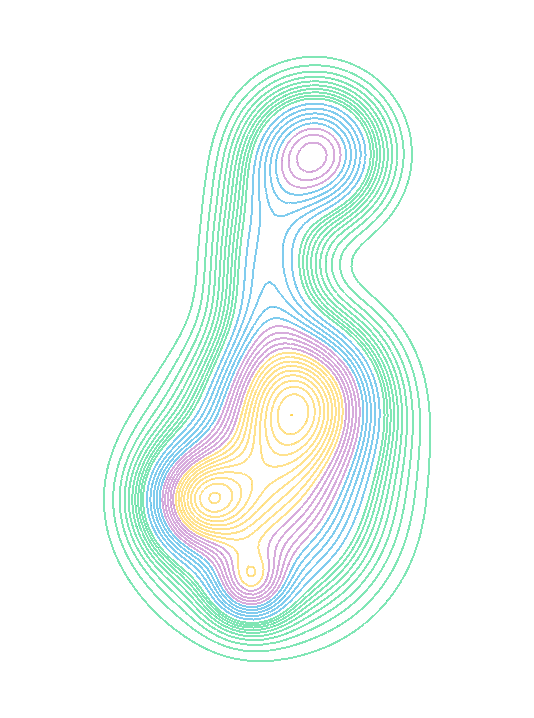
\includegraphics[trim=100 25 75 0, clip, angle=280, scale=0.25]{scripts/figures/scalar_contour.png}
  
\includegraphics[trim=200 200 200 200, clip, width=0.5\textwidth]{scripts/figures/surf/side.png}
  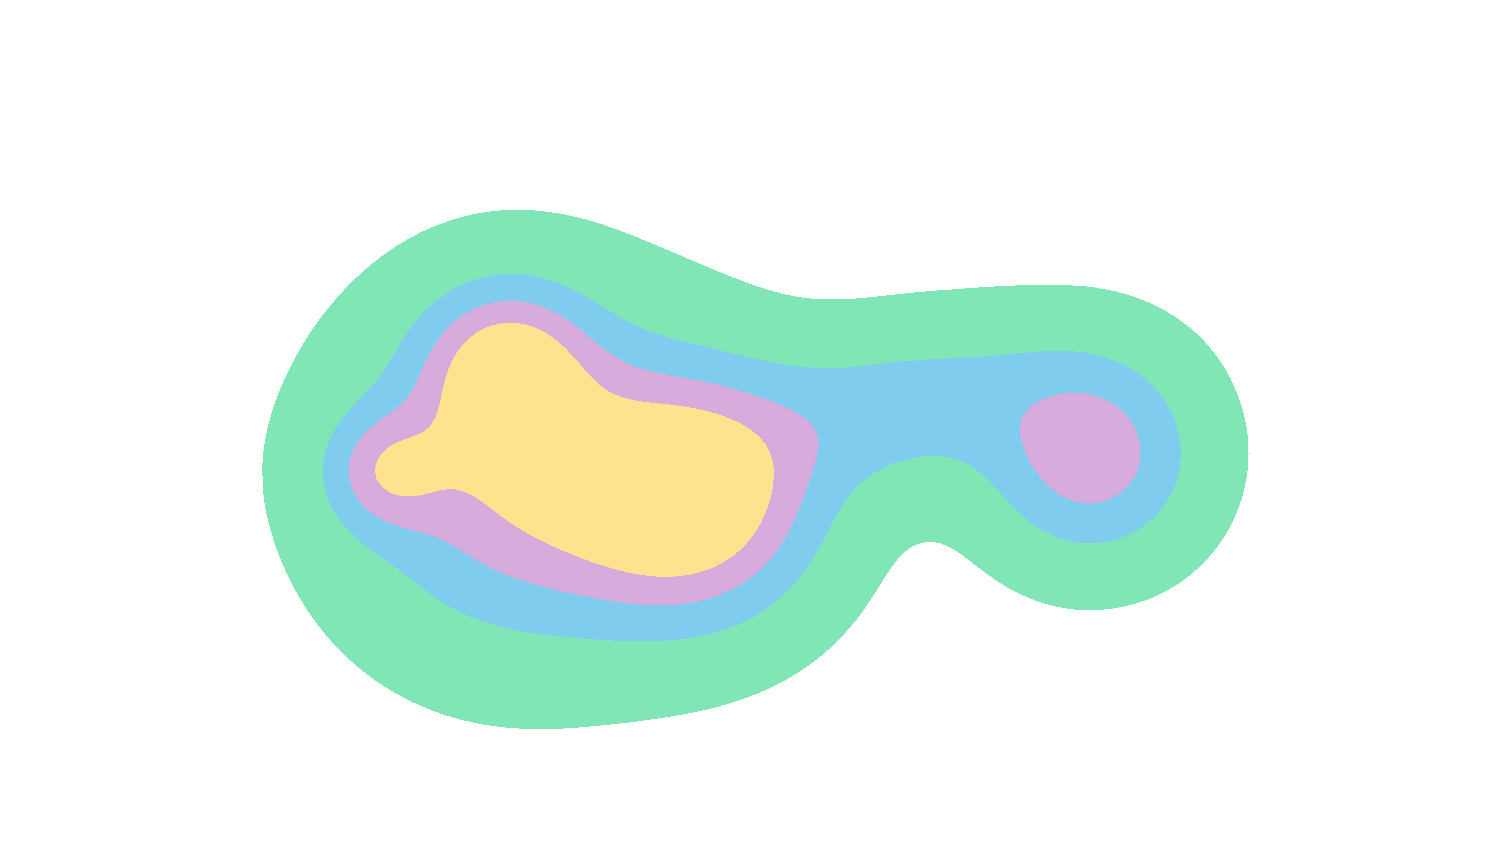
\includegraphics[trim=200 0 200 200, clip, width=0.3\textwidth]{scripts/figures/surf/top.png}
  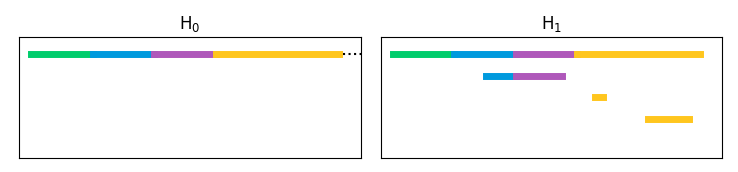
\includegraphics[scale=0.75]{scripts/figures/scalar_barcode_true.png}
  % \includegraphics[trim=0 310 270 0, clip, scale=0.8]{scripts/figures/scalar_restricted.png}
  % \includegraphics[scale=0.55]{scripts/figures/scalar_barcode_super_0.png}
  % \includegraphics[scale=0.55]{scripts/figures/scalar_barcode_sub_1.png}
\end{figure}
